% Template LaTeX document for CSSR4Africa Deliverables
% Adapted from documents prepared by EPFL for the RobotCub project
% and subsequently by the University of Skövde for the DREAM project
%
% DV 28/06/2023

\documentclass{CSSRforAfrica}

\usepackage{array}
\usepackage{caption}
\usepackage{dirtree}
\usepackage{float}
\usepackage{fontenc}
\usepackage{geometry}
\usepackage{graphicx}
\usepackage{latexsym}
\usepackage{listings}
\usepackage{lmodern}
\usepackage{longtable}
\usepackage{pdflscape}
\usepackage{pdfpages}
\usepackage[table,dvipsnames,svgnames]{xcolor}
\usepackage{tikz}
\usepackage[titletoc,title]{appendix}
\usepackage{url}
\usepackage{tabularx,colortbl}
\usepackage{verbatim}
\usepackage{subcaption}
\usepackage{multicol}
\usepackage[hidelinks,colorlinks=false]{hyperref}
\usetikzlibrary{shapes.geometric, positioning, arrows.meta,shapes,arrows, calc}
\captionsetup[figure]{format=hang}
\definecolor{backcolour}{rgb}{0.95,0.95,0.95} 
\definecolor{codegreen}{rgb}{0,0.6,0}
\definecolor{codepurple}{rgb}{0.5,0.0,0.5}
\definecolor{greenyellow}{rgb}{0.8, 0.7, 0.10}

\lstdefinestyle{withoutNumbering}{
    backgroundcolor=\color{backcolour},   
    commentstyle=\color{codegreen},
    keywordstyle=\color{magenta},
    stringstyle=\color{codepurple},
    %%basicstyle=\ttfamily\small,
    basicstyle=\ttfamily\scriptsize,
    breakatwhitespace=false,         
    breaklines=true,                 
    captionpos=b,                    
    keepspaces=true,                 
    showspaces=false,                
    showstringspaces=false,
    showtabs=false,                  
    tabsize=2
}

% Define custom colors
\definecolor{backcolour}{rgb}{0.95,0.95,0.92}
\definecolor{codegreen}{rgb}{0,0.6,0}
\definecolor{codeblue}{rgb}{0,0,0.8}
\definecolor{codepurple}{rgb}{0.58,0,0.82}
\definecolor{darkred}{rgb}{0.6,0,0.0}
\definecolor{brown}{rgb}{0.6,0.4,0.2}

% Define a custom XML language with keywords for different node types
\lstdefinelanguage{XMLCustom}{
    morestring=[b]",
    morestring=[b]',
    morecomment=[s]{<!--}{-->},
    sensitive=true,
    % Control Flow Nodes:
    morekeywords={
      Sequence, Fallback, Parallel, Inverter, RetryUntilSuccessful, KeepRunningUntilFailure, ForceFailure
    },
    % Tree Nodes:
    alsoletter={<},
    morekeywords=[2]{
      root, BehaviorTree, SubTree, START_OF_TREE
    },
}

% Define the style for XML code
\lstdefinestyle{XMLStyle}{
    language=XMLCustom,
    backgroundcolor=\color{backcolour},
    basicstyle=\ttfamily\small,
    %%basicstyle=\ttfamily\footnotesize,
    commentstyle=\color{codegreen},
    keywordstyle=\color{codeblue}\bfseries,
    keywordstyle=[2]\color{brown}\bfseries,
    stringstyle=\color{codepurple},
    breaklines=true,
    breakatwhitespace=true,
    showstringspaces=false,
    captionpos=b,
    escapeinside={(*@}{@*)},
    literate={<}{{\textcolor{darkred}{<}}}1 {>}{{\textcolor{darkred}{>}}}1 {</}{{\textcolor{darkred}{</}}}2
}



\hypersetup{
    colorlinks=true,
    linkcolor=black,
    filecolor=magenta,      
    urlcolor=blue,
    citecolor=blue,
    pdfpagemode=FullScreen
    }


\newcommand{\blank}{~\\}
\newcommand{\checkbox}{{~~~~~~~\leavevmode \put(-7,-1.5){  \huge $\Box$  }}}


 
%% Directory Tree Font
%\renewcommand*\DTstyle{\rmfamily\footnotesize}
%\renewcommand*\DTstyle{\sffamily\footnotesize}
%\renewcommand{\DTstyle}{\small\ttfamily}
\renewcommand{\DTstyle}{\footnotesize \ttfamily}
%\renewcommand{\DTstyle}{\scriptsize \ttfamily}

\captionsetup[figure]{format=hang}

\begin{document}
\input{epsf}

%%
%% SHOULD NOT NEED TO BE CHANGED BEFORE THIS POINT
%% ------------------------------------------------
%%

\deliverable{D6.2}              
\title{6.2  Use Case Evaluation}   

\leadpartner{Carnegie Mellon University Africa (for Wits)}      
\partner{Carnegie Mellon University Africa}                               

\revision{1.2}                           
\deliverabledate{30/06/2025}  
\submissiondate{13/06/2025}  
\revisiondate{16/06/2025}      
\disseminationlevel{PU}
\responsible{D. Vernon }       


%%
%% Create the titlepage
%%

\maketitle
 

\section*{Executive Summary}
%===============================================================
\label{executive_summary}
%%\addcontentsline{toc}{section}{Executive Summary}
 
Deliverable D6.2 documents the outcome of Task 6.2, i.e., the  evaluation of the  robot laboratory tour guide use case defined in Work Package WP2, and implemented using the outcomes of WP1 - WP5, i.e., using the cultural knowledge, the scenario specification, and the integrated  robot's sensory and interaction capabilities. The purpose of the evaluation is to identify  any required changes in the CSSR4Africa system architecture,  its constituent ROS nodes, and its knowledge bases.  These changes  are to be implemented in Tasks  1.5, 2.4, 3.6, 4.4, and 5.6, all of which are ``Use Case Feedback'' tasks. 

In addition to evaluating the implementation using the Robot Social Attribute Scale (RoSAS) \cite{Carpinellaetal2017}, as originally specified in the work plan,  we also address the system engineering issues that arise when the  individual ROS nodes worked collectively as a complete system to deliver the  functionality required in the use cases, either because of incorrect use of each nodes topics and services, or because the resultant behavior does not match expectations.   This latter evaluation was inadvertently omitted from the work plan, but is included here since this functionality is dependent on the robot mission associated with a particular user case.

In summary, there are two elements of evaluation, the first addressing the purely functional aspects of successfully carrying out the robot mission, and the second addressing the user's perception from a social perspective of the manner in which the mission is executed, i.e., an evaluation using RoSAS.

Note: the work plan assigns responsibility for this deliverable to the University of the Witswatersrand. However, for reasons explained in the following, the material in this report was developed and written by the team at Carnegie Mellon University Africa. Since this involved a significant amout of additional, unplanned effort, only one use case, the laboratory tour, has been implemented to date, leaving the second use case, the receptionist, to be implemented later. 
  
\pagebreak
\tableofcontents
\newpage


\section{Introduction}
%===============================================================
 \label{section:introduction}

  
Deliverable D6.2 documents the outcome of Task 6.2, i.e., the  evaluation of the  use cases defined in Work Package WP2, implemented using the outcomes of WP1 - WP5, i.e., the cultural knowledge, the scenario specification, and the integrated  robot's sensory and interaction capabilities. 

The use cases are captured using the robot mission specification methodology documented in Deliverable D5.4.2 Robot Mission Language, i.e., using behavior trees \cite{Ghzoulietal2023,DortmansPunter2022}. The resultant behavior tree provides the input to the {\small \tt behaviorController} ROS node documented in Deliverable D5.4.3.  Running the {\small \tt cssr\_system} ROS package against the behavior tree robot mission specification provides a demonstration of the complete working system for the corresponding  use case. 

In the work plan, the objective of this task is to evaluate the implementation using the Robot Social Attribute Scale (RoSAS)  \cite{Carpinellaetal2017} and produce a set of required adjustments for the interaction primitives and design patterns.  It was planned to then implement these adjustments in Tasks  1.5, 2.4, 3.6, 4.4, and 5.6, all of which are ``Use Case Feedback'' tasks. This plan assumed that the software that was integrated into the CSSR4Africa system, i.e., accepted for inclusion in the CSSR4Africa software repository in Task 3.5 after having demonstrated compliance with the CSSR4Africa software engineering standards documented in D3.4, would operate successfully as a system.   As such, it neglected to allow for the almost inevitable eventuality that issues would arise when the   individual ROS nodes worked collectively as a complete system, either because of incorrect use of each nodes topics and services, or because the resultant behavior does not match expectations.    In effect, the work plan omitted the systems engineering element of system integration in Task 3.5, ensuring that the entire system operated correctly to deliver the desired  functionality. Since this functionality is dependent on the robot mission associated with a particular user case, the scope of this deliverable has been broadened to address this system engineering aspect of system integration,  with two elements of evaluation, the first addressing the purely functional aspects of successfully carrying out the robot mission, and the second addressing the user's perception from a social perspective of the manner in which the mission is executed, i.e., an evaluation using RoSAS.

Note: responsibility for this deliverable in the  work plan is assigned to the University of the Witswatersrand. However, the work documented in this report was undertaken by CMU-Africa. This was necessary because, due to extensive delays in the delivery of the Pepper robot to the University of the Witswatersrand, little or no progress had been made on this and six other essential tasks assigned to the University of the Witswatersrand: Task 5.4.1 Cultural Knowledge Ontology \& Culture Knowledge Base, Task 5.4.2 Robot Mission Language, Task 5.4.3 Robot Mission Interpreter, Task 5.5.2.1 English Text to Speech Conversion, Task 5.5.4.2 Integrated  Text to Speech Conversion, and Task 6.1 Use Case Implementation.  Consequently,  CMU-Africa took joint responsibility for these seven deliverables.  Since this involved a significant amout of additional, unplanned effort, only one use case, the laboratory tour,  has been implemented to date, leaving the second use case, the receptionist, to be implemented later.


\section{Evaluation of the Functional Operation of the CSSR4Africa System}
%===============================================================
 \label{section:functional_evaluation}

The first element of the use case evaluation addresses the  purely functional aspects of successfully carrying out the robot mission, requiring the integration of all twelve ROS nodes in the system architecture documented in Deliverable D3.1.  This integration was accomplished in an incremental manner, progressively introducing additional ROS nodes, in two phases.  The first phase used software that was functionally complete, at least concerning the specification in the work plan, but some of which was not yet compliant with the software engineering standards set out in Deliverables D3.2 Software Engineering Standards Manual and Deliverable D3.4 System Integration and Quality Assurance Manual.  The second phase used software that is compliant and is available in the public CSSR4Africa \href{https://cssr4africa.github.io/software}{GitHub and HuggingFace repositories}.   We adopted this approach to avoid unecessary delays in assessing the functionality of the individual ROS nodes.  The evaluation in this report is based on the integration in the first phase.  

Table \ref{table:phase1a} lists the  changes that have been identified in the first phase of the evaluation and implemented prior to the start of Tasks  1.5, 2.4, 3.6, 4.4, and 5.6 (Use Case Feedback) on July 1, 2025.

Table \ref{table:phase1b} lists the  changes that have been identified in the first phase of the evaluation, and are scheduled for implementation in Tasks  1.5, 2.4, and 3.6 during the first three months of the final year of the project, and in Tasks 4.4 and 5.6 during the first nine months of the final year.

 It is expected that there will be no significant differences in the evaluation using software integrated in the second phase, apart from the elimination of the issues identified in Table \ref{table:phase1a}.

\begin{center}
\begin{table}[H]
\begin{tabularx}{\linewidth}{| l | l | X |}
\hline 
{\small Task No.}                               & {\small Node }                                                 &  {\small Change}       \\
\hline
{\footnotesize 5.4.3 }  & {\footnotesize \verb+behaviorController+}     & {\footnotesize Do not request \verb+overtAttention+ to change to social mode after establishing mutual gaze with the visitor.   } \\ 
\hline
{\footnotesize 5.4.3  }  & {\footnotesize \verb+behaviorController+}     & {\footnotesize  Prompt the user before traversing a behavior tree for the first time.} \\ 
\hline
{\footnotesize 5.4.3  }  & {\footnotesize \verb+behaviorController+}     & {\footnotesize  Prompt the user after the initial traversal of the behaviorTree to determine whether to quit or traverse again.} \\ 
\hline
{\footnotesize 5.4.3}  & {\footnotesize \verb+behaviorController+}     & {\footnotesize  Unit tests should support testing different execution paths within the mission specification (behavior tree). A new configuration file key should enable selection among four partial paths and a complete path.} \\ 
\hline
{\footnotesize 5.4.3 }  & {\footnotesize \verb+behaviorController+}     & {\footnotesize  Speak the name of each action and condition node as they is being traversed during execution. The option should be provided as a configuration key.} \\ 
\hline
{\footnotesize 5.4.3 }  & {\footnotesize \verb+behaviorController+}     & {\footnotesize  Adapt  to include blocking behavior for a duration proportional to the number of words, ensuring that utterances are completed before the next step proceeds.} \\ 
\hline
{\footnotesize 5.4.3 }  & {\footnotesize \verb+behaviorController+}     & {\footnotesize  After issuing a service request to textToSpeech in English, block (or simulate blocking behavior) until the utterance is complete.} \\ 
\hline
\end{tabularx}
\caption{Required changes that have been identified in the first phase of the evaluation of the functional operation of the CSSR4Africa system, i.e., during system integration of ROS nodes. These changes have been implemented  prior to the start of Tasks  1.5, 2.4, 3.6, 4.4 and 5.6 (Use Case Feedback) on July 1, 2025. The task number refers to the task that is responsible for implementing the change.}
\label{table:phase1a}
\end{table}
\end{center}


\begin{center}
\begin{table}[H]
\begin{tabularx}{\linewidth}{| l | l | X |}
\hline 
{\small Task No.}                               & {\small Node }                                                 &  {\small Change}       \\
\hline
{\footnotesize 2.4 }  & {\footnotesize \verb+behaviorController+}     & {\footnotesize Have two variants of the lab tour use case: (a) the robot operates autonomously, without requiring someone to introduce it, and (b) someone introduces Pepper and initiates the tour demo.    The former requires the Pepper robot to locate a visitor, wait until mutual gaze is established, and then ask the visitor if she or he would like a tour. The second omits this part, launches directly into the tour, and doesn't require the visitor to follow the robot.} \\ 
\hline
{\footnotesize 5.6 }  & {\footnotesize \verb+behaviorController+}     & {\footnotesize Minimize pauses or dead zones between different phases of the tour, i.e., between each behavior tree action nodes.   } \\ 
\hline
{\footnotesize 4.4 }  & {\footnotesize \verb+behaviorController+}     & {\footnotesize  Ensure that visitor does not have to facilitate interaction by standing is a particular position.} \\ 
\hline
{\footnotesize 5.6 }  & {\footnotesize \verb+behaviorController+}     & {\footnotesize  Improve navigation and locomotion, to make it look more purposeful, e.g., using  the divide-and-conquer algorithm.} \\ 
\hline
{\footnotesize 5.6 }  & {\footnotesize \verb+behaviorController+}     & {\footnotesize  Implement more comprehensive failure handling.} \\ 
\hline
{\footnotesize 5.6 }  & {\footnotesize \verb+behaviorController+}     & {\footnotesize  Query the culture knowledge base for the deicticHand key-value pair and pass the value to \verb+gestureExecution+.} \\ 
\hline
{\footnotesize 5.6 }  & {\footnotesize \verb+behaviorController+}     & {\footnotesize  Query the culture knowledge base for the eyeContactDuration  and nodExtentRespect key-value pairs and pass the value to \verb+overtAttention+.} \\ 
\hline
{\footnotesize 5.6 }  & {\footnotesize \verb+behaviorController+}     & {\footnotesize  Implement the receptionist use case.}\\ 
\hline
{\footnotesize 5.6 }  & {\footnotesize \verb+speechEvent+}     & {\footnotesize  Improve the automatic speech recognition, both in terms of reducing the time taken and the reliability.} \\ 
\hline
{\footnotesize 5.6 }  & {\footnotesize \verb+speechEvent+}     & {\footnotesize  Allow more natural spoken interaction by the visitor.} \\ 
\hline
{\footnotesize 5.6 }  & {\footnotesize \verb+overtAttention +}     & {\footnotesize  Adapt  seek mode to adhere to cultural norms by dropping the head slightly intermittently to avoid looking at a visitor continuously for long periods. The duration of the mutual gaze before dropping the head and the extent of  the drop should be determined by the \verb+behaviorController+ by quering the culture knowledge base using the eyeContactDuration  and nodExtentRespect key-value pairs.} \\ 
\hline
{\footnotesize 5.6 }  & {\footnotesize \verb+gestureExecution+}     & {\footnotesize Add or extend a service to use a key-value pair \verb+deicticHand LEFT+ $\mid$ \verb+RIGHT+ $\mid$ \verb+EITHER+. } \\ 
\hline
{\footnotesize 5.6 }  & {\footnotesize Cultural knowledge base}     & {\footnotesize  Add a key-value pair (\verb+deicticHand LEFT+ $\mid$ \verb+RIGHT+ $\mid$ \verb+EITHER+) to the culture knowledge base.  } \\ 
\hline
{\footnotesize 4.4, 5.6 }  & {\footnotesize All nodes}     & {\footnotesize  Implement  a means of resetting the node through a service call.} \\
%%This will allow a script to reset all nodes using the ROS rosservice command line interface. 
%%This will avoid having to kill all active ROS nodes and re-launch to entire system in the case of fatal failure of the system.} \\ 
\hline
\end{tabularx}
\caption{Required changes that have been identified in the first phase of the evaluation of the functional operation of the CSSR4Africa system, i.e., during system integration of ROS nodes. These changes are scheduled for implementation in Tasks  1.5, 2.4, 3.6,  4.4 and 5.6 in the final year. The task number refers to the task that is responsible for implementing the change.}
\label{table:phase1b}
\end{table}
\end{center}



\section{Evaluation of the Social Behaviors of the CSSR4Africa System}
%===============================================================
 \label{section:social_evaluation}

The second element of the use case evaluation addresses the  user's perspective  (i.e., the perspective of the visitor being given a tour of the lab by the robot). It focusses on  the user's perception of the robot's socio-cultural behavior when carrying out the robot mission.  This is accomplished using the  Robot Social Attribute Scale (RoSAS) \cite{Carpinellaetal2017}.

Since, at time of writing, the only cultural knowledge (documented in Deliverable D5.4.1) that is used in the use case demonstration are the verbal interaction key-value pairs.  The non-verbal and spatial interaction cultural knowledge has not yet been deployed. As noted in Table \ref{table:phase1b},  it is planned to do this in the final year of the project.  Since RoSAS focuses mainly on appearance, we limit our evaluation in this section to an assessment of the impact of using biological motion when performing non-verbal gestures.  The material that follows is taken directly from CSSR4Africa paper in the Journal of Humanoid Robotics \cite{AkinadeBarrosVernon2025}.  A more complete RoSAS evaluation will be carried out at the end of the project in Task 6.3 Use Case Re-Evaluation.

\subsection{Evaluation of User Perception of Biological Motion in Deictic Gestures}
%--------------------------------------------------------------------


\begin{figure}
    \centering
    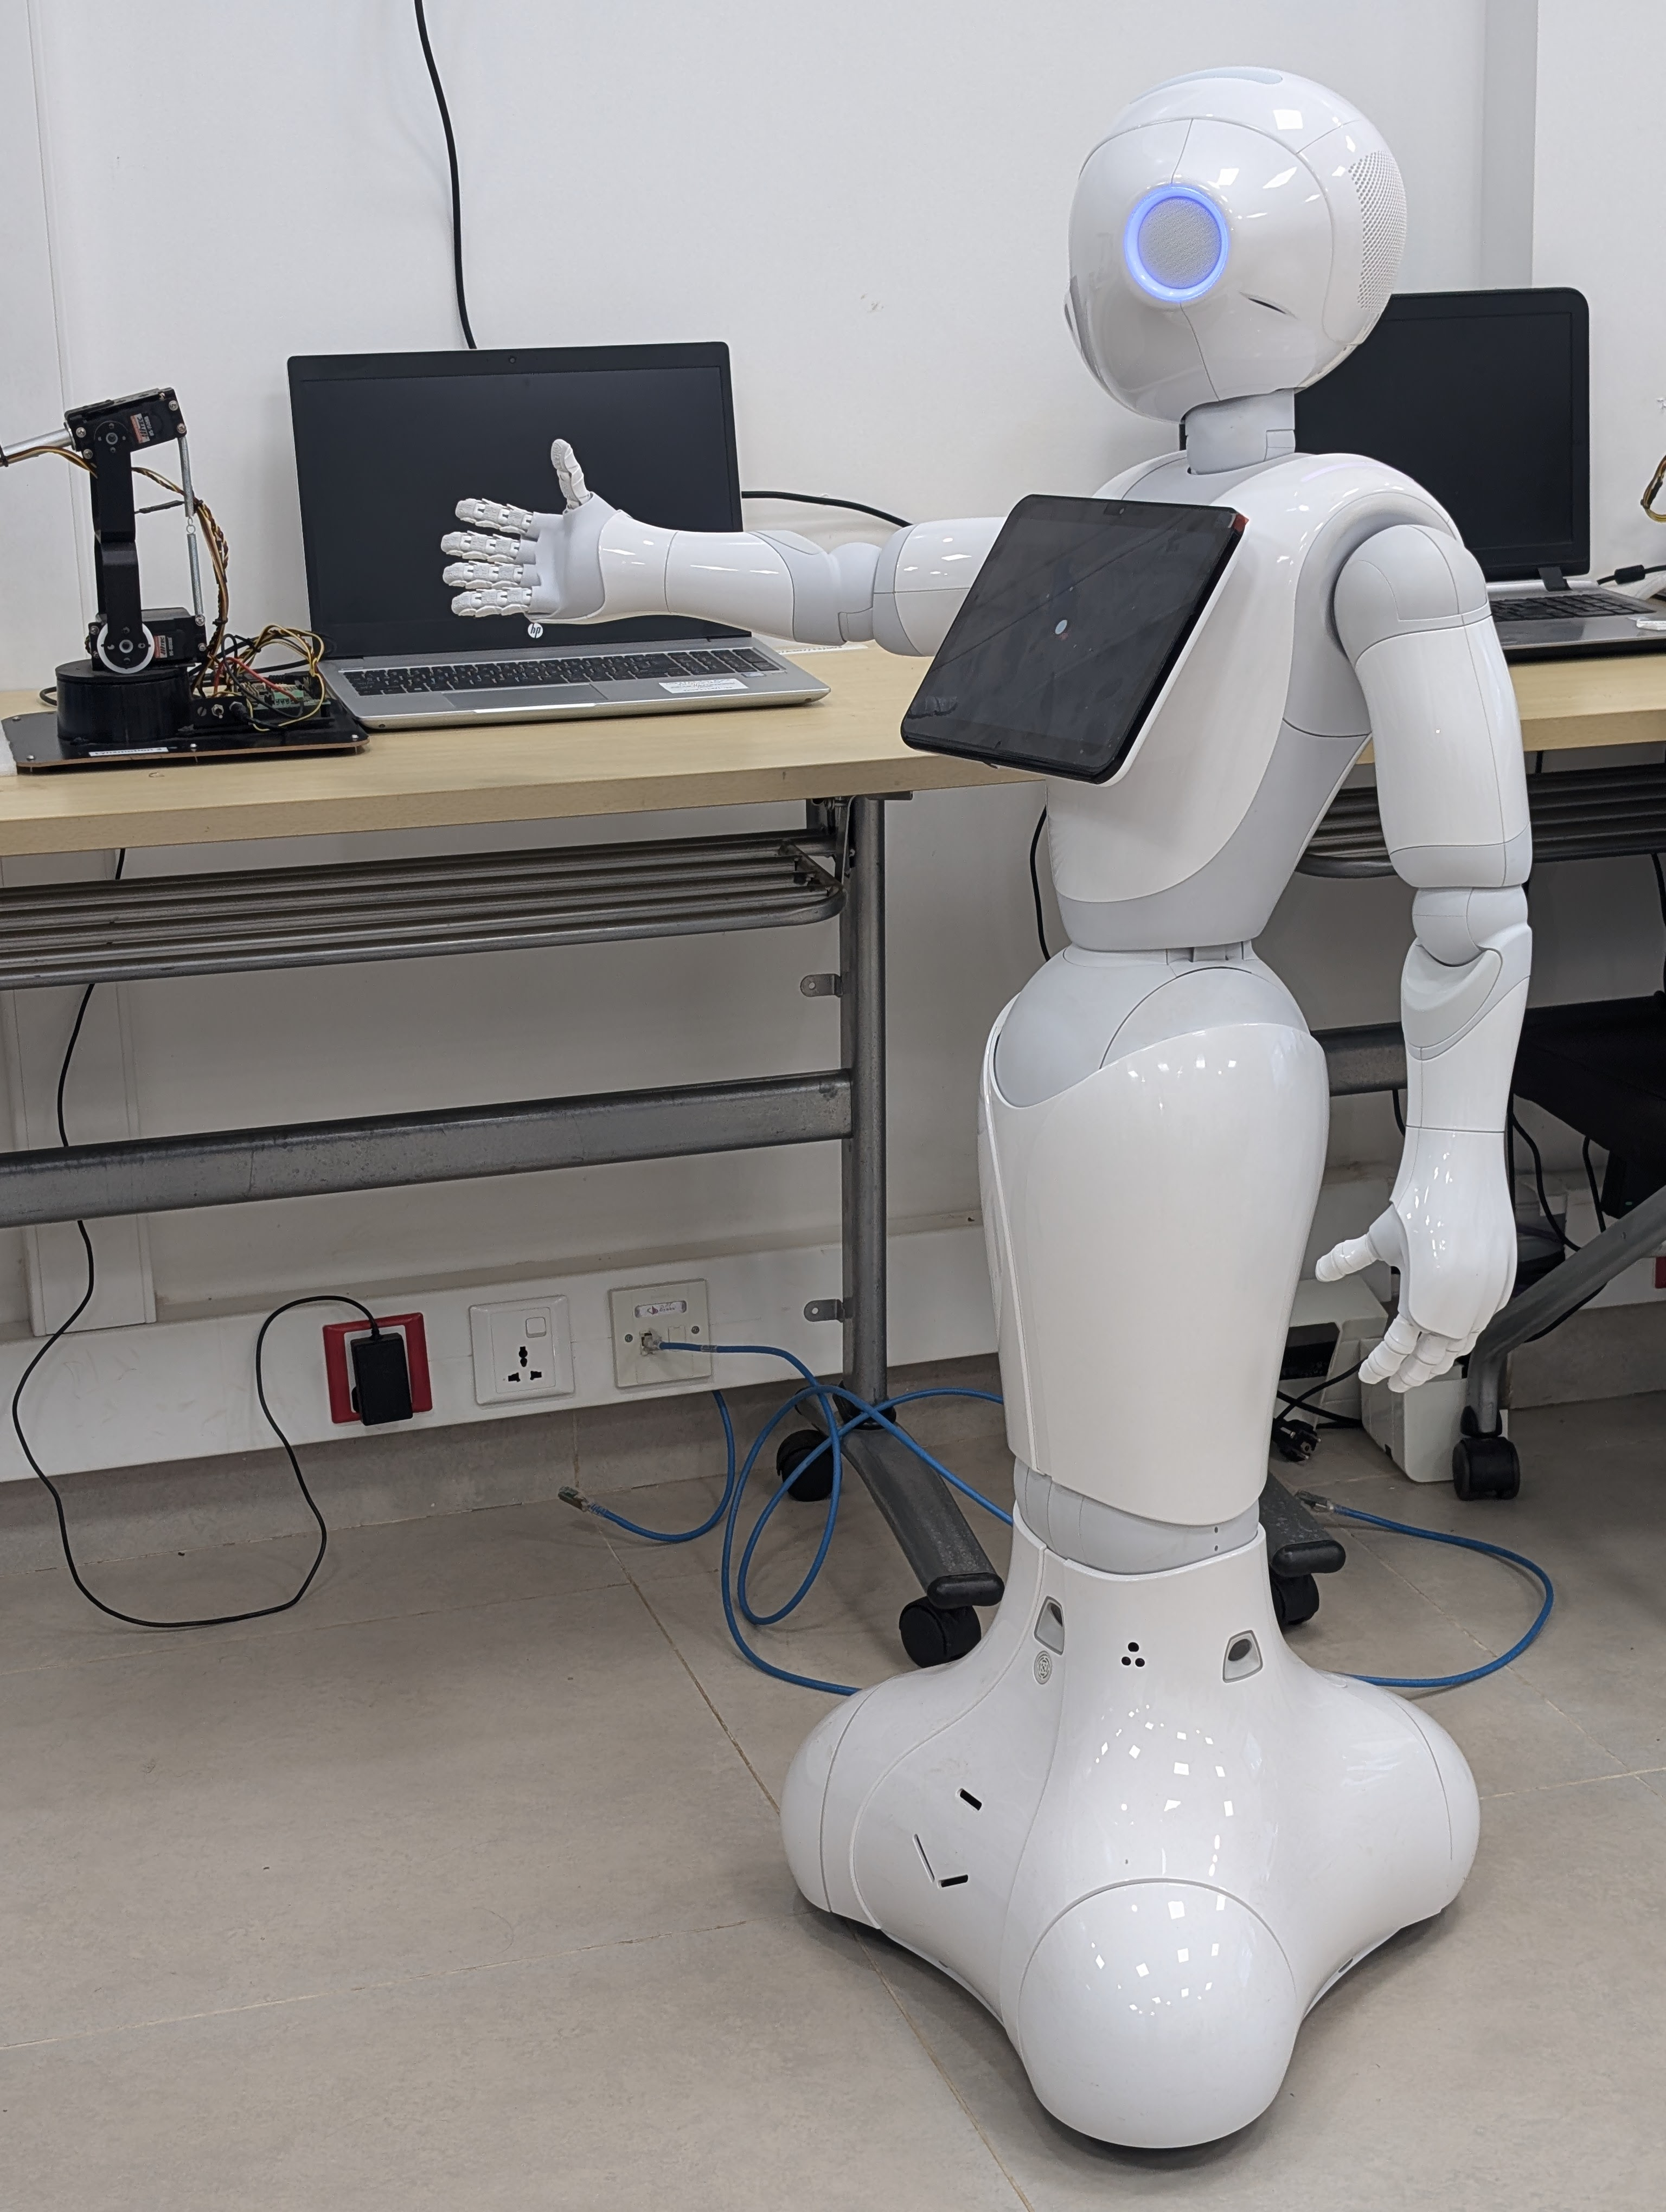
\includegraphics[width=0.4\textwidth]{Pepper_Gesture.jpg}
    \caption{The Pepper robot performing a deictic pointing gesture during the experiment. Note that the robot's gaze is directed to the object to which it is gesturing. The picture is taken from the perspective of the user in the study.}
    \label{fig:Pepper_Gesture}
\end{figure}

The aim is to evaluate the impact of biologically inspired motion on the perceived social attributes of the Pepper humanoid robot. This was achieved through a controlled user study where participants observed the robot executing gestures using two distinct motion profiles: biological and non-biological (trapezoidal). The evaluation employed the Robotic Social Attributes Scale (RoSAS), a well-established tool in social robotics research, to assess dimensions of warmth and discomfort, which are critical for understanding human-robot interaction dynamics \cite{Carpinellaetal2017,Spatola2021,Mandletal2022,Jorgensen2021}.

In this study, seventeen participants (seven females and ten males), who were graduate students at Carnegie Mellon University Africa in Rwanda, were recruited and exposed to a within-subjects experimental design. Each participant observed the Pepper robot perform a deictic gesture executed under two conditions: (1) a trapezoidal motion profile, which lacked the smoothness and natural characteristics of biological motion, and (2) a biological motion profile, which utilized the minimum jerk model to mimic natural human movement. Figure \ref{fig:Pepper_Gesture} shows the Pepper robot performing a gesture during the experiment. The study followed a within-subjects design, where each participant was exposed to two experimental conditions, without prior knowledge of what the gestures executed in each conditions entailed. It is important to note that nine of the participants had no prior experience working with humanoid robots, while the other eight had some experience.


The order of the conditions was randomly assigned to participants to mitigate potential order effects. Participants were randomly assigned to either observe the gestures executed using biological motion first, followed by the control gestures, or vice versa. As a result, ten of the participants observed the trapezoidal motion profile first, while the other seven participants observed the biological motion profile first.

After observing the robot's gestures in each condition, participants were asked to complete a survey based on  RoSAS. The survey instrument consisted of nineteen questions, with eleven questions evaluating the warmth dimension and eight questions assessing the discomfort dimension. The warmth dimension encompassed attributes like naturalness, fluidity, expressiveness, and friendliness, while discomfort captured impressions such as awkwardness, unease, and unnaturalness. Participants rated their perceptions using a seven-point Likert scale (1 = strongly disagree, 7 = strongly agree).

This experimental design enabled a direct comparison of human perception of the robot’s gestures under both motion profiles. By analyzing participants’ responses, the study sought to determine whether biologically inspired motion enhanced the perceived warmth of the robot and reduced discomfort, thereby advancing our understanding of how motion profiles influence social perceptions of humanoid robots. The evaluation framework builds on previous applications of RoSAS in social robotics, which have demonstrated its utility in measuring social traits like anthropomorphism, competence, and engagement across diverse contexts and cultural settings \cite{Scassellatietal2012,Oliveiraetal2021}.


\subsection{Results}
%----------------

\subsection{User Response Evaluation}
This section presents an analysis of the survey data collected to evaluate the impact of biologically inspired gestures on the perceived social attributes of the Pepper robot, focusing on the warmth and discomfort dimensions as measured by the Robotic Social Attributes Scale (RoSAS). 
We begin by outlining the statistically significant differences observed between the two gesture profiles (biological and trapezoidal), specifying the significance levels for each comparison. 
Box plots were generated to illustrate the mean and standard deviation of user responses, offering insights into the relative impact of motion profiles on perceived robot attributes. The overall comparison of the means obtained from the two conditions in both the warmth and discomfort is show in Figure \ref{figure:Overall_means} below. This figure provides a general view of user preferences relative to the neutral point\footnote{The neutral point is $4.0$ on the scale.} on the scale, highlighting differences between the motion profiles.  The biological motion profile (represented in shades of green) demonstrates higher ratings above the midpoint for warmth and lower ratings below the midpoint for discomfort compared to the trapezoidal motion profile (represented in shades of red).


%\begin{figure}[h!]
\begin{figure}[t]
  \centering 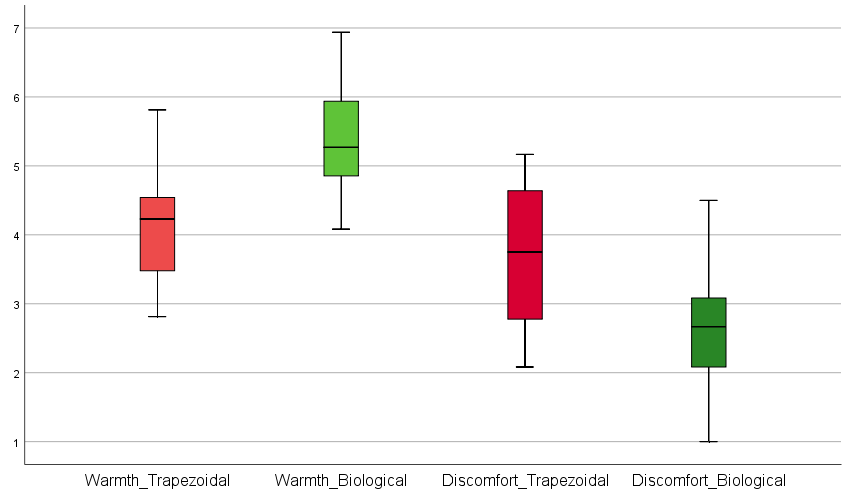
\includegraphics[scale=0.35]{Overall_Means.png}
  \caption{{Mean of Responses in the Warmth and Discomfort Dimensions of  Condition 1 (non-biological control gesture) and Condition 2 (biological motion profile).}}
  \label{figure:Overall_means}
\end{figure}
%The results are organized into three key figures:
%
%Figure Z: Comparison of the overall Warmth and Discomfort dimensions across trapezoidal and biological motion profiles. This figure provides a general view of user preferences and highlights statistically significant differences between the motion profiles, with the biological motion profile showing higher warmth and lower discomfort.
%
%Figure Z+1: Mean and standard deviation of the individual aspects of the Warmth dimension (Naturalness, Fluidity, Expressiveness, and Perceived Friendliness) for trapezoidal and biological motion profiles. This figure highlights how the biological motion profile consistently scored higher across all sub-dimensions, indicating smoother and more human-like motion execution.
%
%Figure Z+2: Mean and standard deviation of the individual aspects of the Discomfort dimension (Awkwardness, Uncertainty, and Unnaturalness) for trapezoidal and biological motion profiles. This figure reveals lower ratings of discomfort in biological motion, demonstrating its ability to evoke a more positive perception of the robot's behavior.

%%\vspace{-6mm}
\subsubsection{Warmth Dimension Analysis}
%- - - - - - - - - - - - - - - - - - - - - - - - 
The overall warmth dimension for the two experiments was analyzed based on four aspects: {\em naturalness}, {\em fluidity of motion}, {\em expressiveness of gestures}, and {\em perceived friendliness of the robot}. 
 
The results for the warmth dimension under the Trapezoidal velocity profile revealed a mean score of 4.14 ($SD$\footnote{$SD$: standard deviation.} $= 0.86$, $SE$\footnote{$SE$: standard error.} $ = 0.21$). The analysis showed no statistically significant difference from the midpoint ($t(16) = 0.664$, $p = 0.516$), with a mean difference of 0.14 and a 95\% confidence interval ranging from $-0.30$ to $0.58$. These findings suggest that the Trapezoidal profile elicited a moderate perception of warmth, but the result was not significantly higher than the neutral point.
In contrast, the Biological motion profile achieved a higher mean score of 5.38 ($SD = 0.83$, $SE = 0.20$). The difference from the midpoint was statistically significant ($t(16) = 6.89$, $p < 0.001$), with a mean difference of 1.38 and a 95\% confidence interval ranging from 0.96 to 1.80.  These findings indicate that participants rated the Biological motion profile as significantly above the neutral point on the warmth dimension.

The mean of the aspects of the warmth dimension under both conditions is shown in Figure \ref{figure:Warmth_means} below. This figure highlights how the biological motion profile  (in shades of green) consistently scored higher across all sub-dimensions than the trapezoidal motion profile (in shades of red), indicating smoother and more human-like motion execution.
%\begin{figure}[h!]
\begin{figure}[t]
  \centering 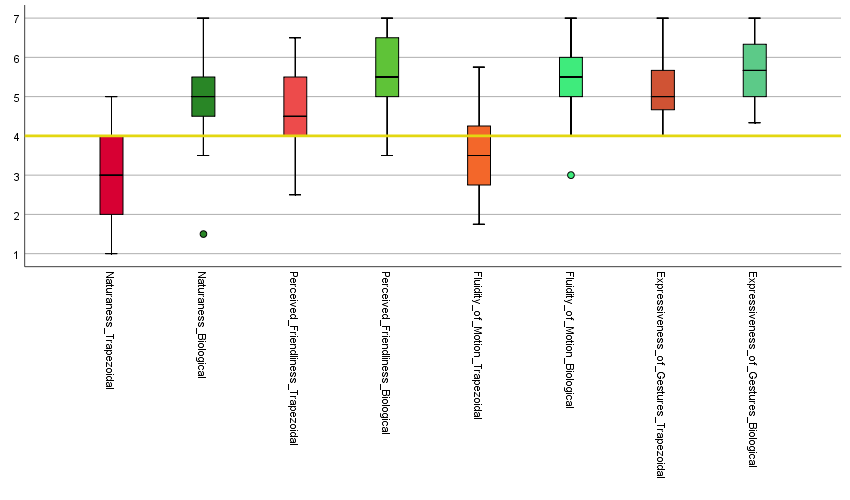
\includegraphics[scale=0.45]{Warmth_Means.png}
  \caption{Mean of Responses of Different Aspects in the Warmth Dimension of  Condition 1 (non-biological control gesture) and Condition 2 (biological motion profile).}
  \label{figure:Warmth_means}
\end{figure}

%\newpage
\vspace{-2mm}
~\\
\noindent \textbf{Naturalness:} 
For the Trapezoidal velocity profile, the Naturalness score was relatively low, with a mean of 3.06 ($SD = 1.16$, $SE = 0.28$). The analysis revealed a significant difference from the midpoint ($t(16) = -3.35$, $p = 0.004$), with a mean difference of $-0.94$ and a 95\% confidence interval of $-1.54$ to $-0.35$. These results suggest that the Trapezoidal motion profile was perceived as significantly less natural than the neutral point.
In comparison, the Biological motion profile scored substantially higher, with a mean of 5.03 ($SD = 1.33$, $SE = 0.32$). The analysis showed a significant difference from the midpoint ($t(16) = 3.20$, $p = 0.006$), with a mean difference of 1.03 and a 95\% confidence interval of 0.35 to 1.71.  These findings indicate that the Biological motion profile was perceived as significantly more natural than the neutral point.
These results demonstrate that the Biological motion profile aligns more closely with participants’ expectations of naturalness, as indicated by its positive deviation from the neutral midpoint. This finding reinforces the idea that biologically inspired motion enhances the perceived realism and smoothness of robot gestures.

\vspace{-2mm}
~\\
\noindent \textbf{Fluidity of Motion:}
The Trapezoidal motion profile resulted in a mean score of 3.51 ($SD = 1.18$, $SE = 0.29$). The analysis showed no statistically significant difference from the midpoint ($t(16) = -1.69$, $p = 0.11$), with a mean difference of $-0.49$ and a 95\% confidence interval spanning from $-1.09$ to $0.12$. These findings suggest that the Trapezoidal motion profile did not strongly convey fluidity.  These findings suggest that the Trapezoidal motion profile did not strongly convey fluidity relative to a neutral perception.
In contrast, the Biological motion profile achieved a significantly higher mean score of 5.38 ($SD = 1.04$, $SE = 0.25$). The analysis revealed a significant difference from the midpoint ($t(16) = 5.51$, $p < 0.001$), with a mean difference of 1.38 and a 95\% confidence interval of 0.85 to 1.91.  These results indicate that the Biological motion profile effectively conveyed a sense of fluidity, exceeding the neutral point by a meaningful margin. 
The Biological motion profile was rated significantly higher in fluidity compared to the Trapezoidal profile. This result underscores the importance of fluid motion in achieving natural and smooth gestures.


\vspace{-2mm}
~\\
\noindent \textbf{Expressiveness of Gestures:}
The Trapezoidal velovity profile scored a mean of 5.27 ($SD = 0.77$, $SE = 0.19$). The analysis revealed a significant deviation from the midpoint ($t(16) = 6.86$, $p < 0.001$), with a mean difference of 1.27 and a 95\% confidence interval of 0.88 to 1.67. These findings indicate that the Trapezoidal motion profile conveyed a high level of expressiveness  relative to a neutral perception.
Similarly, the Biological motion profile achieved an even higher mean score of 5.61 ($SD = 0.81$, $SE = 0.20$). The analysis showed a significant difference from the midpoint ($t(16) = 8.19$, $p < 0.001$), with a mean difference of 1.61 and a 95\% confidence interval of 1.19 to 2.02. This demonstrates that the Biological profile was also highly expressive, significantly exceeding the neutral point.
Both motion profiles were rated as highly expressive when compared to the neutral midpoint. These findings suggest that both profiles are effective in conveying expressiveness in robot gestures, with the Biological motion profile showing a slightly higher perceived expressiveness. This result suggests that which may imply that incorporating biological motion profiles may not essentially influence the magnitude of expressiveness shown by the robot while executing the gestures.

 
~\\
\noindent \textbf{Perceived Friendliness of Robot:}
For the Trapezoidal motion profile, the mean score for Perceived Friendliness was 4.12 ($SD = 0.79$, $SE = 0.19$). The analysis revealed no significant difference from the midpoint ($t(16) = 0.643$, $p = 0.529$), with a mean difference of $0.12$ and a 95\% confidence interval of $-0.29$ to $0.53$. These results indicate a neutral perception of friendliness for the Trapezoidal profile.
The Biological motion profile achieved a higher mean score of 5.48 ($SD = 0.84$, $SE = 0.20$). The analysis showed a significant difference from the midpoint ($t(16) = 7.16$, $p < 0.001$), with a mean difference of $1.48$ and a 95\% confidence interval of $1.04$ to $1.91$. These results suggest that the Biological profile significantly enhanced the perception of friendliness compared to the neutral midpoint.
Both profiles were evaluated relative to the midpoint, with the Trapezoidal profile eliciting a neutral response and the Biological motion profile showing a significant positive perception of friendliness.

~\\
\noindent \textbf{Paired t-test:}
In order to understand the actual difference between the warmth dimensions in the two conditions, a paired $t-test$ was conducted between the overall warmth dimension for the linear and biological motion profiles. The results below showed a statistically significant difference $(t = -4.17, p  = 0.001)$, indicating that the biological motion profile was perceived as significantly warmer than the linear velocity profile.
 
These results provide insights into how participants perceived the robot's gestures in terms of warmth, highlighting the effectiveness of the biological motion profile in conveying warmth in human-robot interaction scenarios. The findings that the mean values for the fluidity of motion, naturalness of movement, and perceived friendliness were significantly higher when biological motion was incorporated into the robot's movements have important implications. These results suggest that leveraging biological motion principles can enhance positive user experiences during human-robot interactions. Higher ratings of fluidity and naturalness indicate that biological motion helped the robot's movements appear more aligned with human motion patterns. This increased sense of familiarity and biomimicry can reduce the perception of robots as mechanical, unfamiliar entities, potentially mitigating feelings of discomfort during interactions. 

The higher ratings of perceived friendliness associated with biological motion have significant implications for building positive relationships between humans and social robots. Friendly and approachable demeanours can encourage users to feel more comfortable, engaged, and willing to interact with social robots, potentially increasing acceptance and adoption rates in various application domains.


\subsubsection{Discomfort Dimension Analysis}
%- - - -  - - - - - - - - - - - - - - - - - - - - - 
The overall discomfort dimension for the two Condition was analyzed following three key attributes:{\em perceived unnaturalness}, {\em awkwardness and unease}, and {\em perceived uncertainty}. This dimension is reverse-scored, thus a smaller value for discomfort is interpreted as a better interaction experience. Thus, Condition 2 had better results with lesser discomfort values than Condition 1. 

The Discomfort score for the Trapezoidal motion profile was moderate, with a mean of 3.64 ($SD = 0.99$, $SE = 0.24$). The analysis showed no significant deviation from the midpoint ($t(16) = -1.49$, $p = 0.156$), with a mean difference of $-0.36$ and a 95\% confidence interval spanning from $-0.87$ to $0.15$. This indicates that the Trapezoidal profile did not strongly evoke discomfort but was not significantly lower than the midpoint.
The Biological motion profile yielded a significantly lower discomfort score, with a mean of 2.59 ($SD = 0.86$, $SE = 0.21$). The analysis revealed a significant difference from the midpoint ($t(16) = -6.80$, $p < 0.001$), with a mean difference of $-1.41$ and a 95\% confidence interval ranging from $-1.85$ to $-0.97$. These results demonstrate that the Biological profile effectively minimized discomfort, falling well below the neutral point.
This suggests that biologically inspired gestures contribute to a more positive and less unsettling interaction.

The mean of the aspects of the discomfort dimension under both conditions is shown in Figure \ref{figure:Discomfort_means} below. This figure reveals lower ratings of discomfort in biological motion  (in shades of green) when compared with the trapezoidal motion profile  (in shades of red), demonstrating its ability to evoke a more positive perception of the robot's behavior.
%\begin{figure}[h!]
\begin{figure}[t]
  \centering 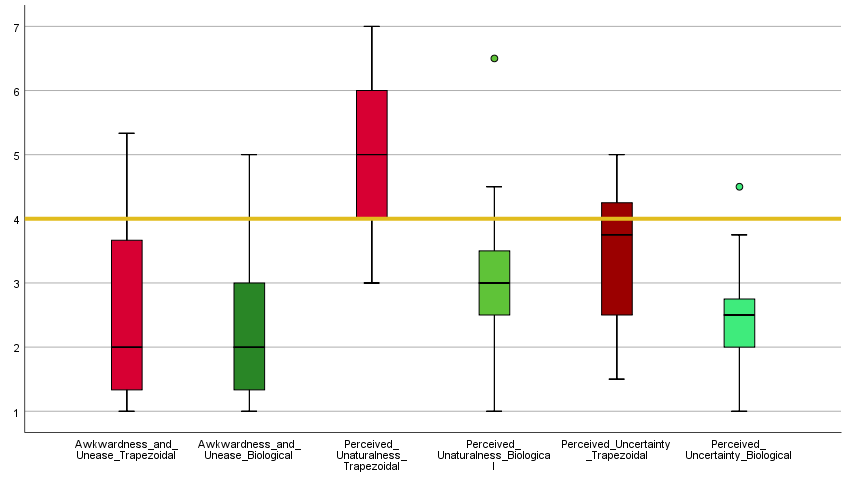
\includegraphics[scale=0.45]{Discomfort_Means.png}
  \caption{Mean of Responses of Different Aspects in the Discomfort Dimension of both Conditions}
  \label{figure:Discomfort_means}
\end{figure}

~\\
\noindent \textbf{Perceived Unnaturalness:} 
Participants rated the unnaturalness of the gestures lower when performed with the biological motion profile (Condition 2) compared to the linear velocity profile. 
For the Trapezoidal motion profile, the mean score for Perceived Unnaturalness was 4.94 ($SD = 1.16$, $SE = 0.28$). The analysis showed a significant deviation from the midpoint ($t(16) = 3.35$, $p = 0.004$), with a mean difference of $0.94$ and a 95\% confidence interval of $0.35$ to $1.54$. These results indicate that the Trapezoidal profile was perceived as unnatural.
In contrast, the Biological motion profile achieved a lower mean score of 2.97 ($SD = 1.33$, $SE = 0.32$). The analysis revealed a significant difference from the midpoint ($t(16) = -3.20$, $p = 0.006$), with a mean difference of $-1.03$ and a 95\% confidence interval of $-1.71$ to $-0.35$. This suggests that the Biological profile was perceived as more natural compared to the neutral midpoint.
Both profiles were analyzed relative to the midpoint of the scale. The Trapezoidal profile was rated as significantly unnatural, while the Biological motion profile was rated as significantly more natural. These results suggest that biologically inspired motion may reduce the perception of unnaturalness in robot movements, as evidenced by the ratings relative to the neutral point. Thus, incorporating a biological motion profile introduces some level of naturalness to the robot's movements. 


~\\
\noindent \textbf{Awkwardness and Unease:}
The biological motion profile was perceived as less awkward and causing less unease than the linear velocity profile. 
The Trapezoidal motion profile resulted in a mean score of 5.53 ($SD = 1.42$, $SE = 0.35$). The analysis revealed a significant difference from the midpoint ($t(16) = -4.26$, $p = 0.001$), with a mean difference of $-1.47$ and a 95\% confidence interval of $-2.20$ to $-0.74$. These results indicate that the Trapezoidal profile evoked significant discomfort. 
The Biological motion profile achieved a substantially lower mean score of 2.31 ($SD = 1.15$, $SE = 0.28$). The analysis showed a significant difference from the midpoint ($t(16) = -6.07$, $p < 0.001$), with a mean difference of $-1.69$ and a 95\% confidence interval of $-2.28$ to $-1.10$. These findings suggest that the Biological profile minimized awkwardness and unease effectively.
Both motion profiles demonstrated significant deviations from the neutral midpoint, This could be due to the appealing physical form of the Pepper humanoid robot \cite{VernonSandini2024}. These results highlight the potential of biologically inspired motion to enhance the perceived smoothness and comfort of robot gestures.

~\\
\noindent \textbf{Perceived Uncertainty:}
Participants rated the gestures as less uncertain or hesitant when performed with the biological motion profile. 
The Trapezoidal motion profile resulted in a mean score of 3.46 ($SD = 1.05$, $SE = 0.25$). The analysis showed a significant difference from the midpoint ($t(16) = -2.14$, $p = 0.049$), with a mean difference of $-0.54$ and a 95\% confidence interval of $-1.08$ to $-0.004$. These findings suggest a moderate level of perceived uncertainty with the Trapezoidal profile.
The Biological motion profile yielded a much lower mean score of 2.49 ($SD = 0.83$, $SE = 0.20$). The analysis showed a highly significant difference from the midpoint ($t(16) = -7.56$, $p < 0.001$), with a mean difference of $-1.51$ and a 95\% confidence interval of $-1.94$ to $-1.09$. These results indicate that the Biological profile effectively minimized uncertainty.
These results highlight the potential of biologically inspired motion to reduce perceptions of uncertainty in robot gestures, suggesting a smoother and more confident movement style when using the Biological motion profile.

~\\
\noindent \textbf{Paired t-test:}
In order to understand the actual difference between the discomfort dimensions in the two conditions, a paired $t-test$ was conducted between the overall discomfort dimension for the linear and biological motion profiles. The results showed a statistically significant difference $(t = 3.972, p  = 0.001)$, indicating that the linear velocity profile was perceived as significantly causing more discomfort than the biological motion profile.

The lower ratings of perceived unnaturalness of movement associated with biological motion indicate that users found the robot's motions to be more lifelike, biomimetic, and aligned with human kinematic profiles. This decrease in unnaturalness can contribute to a heightened sense of familiarity and social presence, facilitating more seamless and engaging interactions. When users perceive a robot's movements as natural and intuitive, they may be more likely to view the robot as a relatable social entity, fostering stronger anthropomorphic perceptions and emotional connections.

The lower ratings of perceived uncertainty associated with biological motion are also noteworthy. Uncertainty in robotic systems can stem from unpredictable or unfamiliar behaviors, which can hinder trust, understanding, and effective communication. By incorporating biological motion cues, which are deeply ingrained in the human perceptual system, \cite{SimionRegolinBulf08} users may have found the robot's actions and intentions more predictable and interpretable, reducing feelings of uncertainty and ambiguity during interactions.

Collectively, these results suggest that adopting biologically inspired motion in social robots can contribute to more natural and potentially more comfortable user experiences. Trajectory analysis of the robot’s arm movements, along with joint state measurements, demonstrates that the biological motion profile more closely aligns with human-like kinematic patterns. Such alignment may improve the predictability and familiarity of the robot's gestures, subtly enhancing the robot's approachability and the user's perception of its social qualities \cite{Vignoloetal2017}.
However, these benefits were observed only in specific aspects, as not all dimensions of user perception showed statistically significant differences between motion profiles. This suggests that while biologically inspired motions offer promising enhancements to robotic behavior, further investigation is needed to understand their impact across diverse social attributes and interaction contexts.
 

\subsection{Summary and Conclusion}
%--------------------------------
This study explored the integration of biologically inspired motion in gestural communication for social robots, with the objective of enhancing the naturalness, expressiveness, and overall quality of human-robot interactions. The motivation stemmed from the growing need for robots to interact with humans in ways that are intuitive, engaging, and aligned with human expectations. By embedding biological motion principles—specifically, the minimum jerk model—into the gestures of a Pepper humanoid robot, this research aimed to improve perceptions of warmth and reduce discomfort during interactions.

The experimental methodology involved implementing a deictic gesture using two distinct motion profiles: a trapezoidal velocity profile and a biologically inspired motion profile. These gestures were executed with the same time duration across both profiles, ensuring comparability while revealing the smoother transitions characteristic of the biologically inspired motion. The user evaluation involved a structured survey based on the Robotic Social Attributes Scale (RoSAS), where participants rated the robot's gestures on dimensions of warmth and discomfort. Quantitative trajectory and joint-state analyses were also performed, using motion capture with an Intel RealSense camera and ArUco markers, to validate the accuracy and consistency of the robot’s motions.

The results demonstrated that gestures executed with the biologically inspired profile were perceived as more natural and fluid, contributing to higher warmth ratings and reduced discomfort in specific dimensions compared to the trapezoidal profile. Statistical analyses revealed significant differences in perceptions for some attributes, while others remained comparable. Motion analysis further confirmed that the biological profile aligns more closely with human kinematics, showing smoother trajectories and fewer abrupt transitions, which are likely to contribute to positive social perceptions.

With a view to widening the breadth of the study described in this report, we plan on running more in-person studies with a copresent robot, and we are also exploring the possibility of conducting studies online using videos, i.e., using a telepresent robot. Li \cite{Li2015} has shown that users perceive copresent robots more positively than telepresent robots, while Donnermann et al. \cite{Donnermannetal2024}  found that there are no significant differences between video presentations and physically present robots in user studies of robots acting as tutors. Both approaches have advantages and limitations, e.g., the greater reach of online studies vs. the immediacy of in-person studies.  Since we are primarily concerned here with the perception of gestures where the robot hands move in three dimensions, and not just in the efficacy of the interaction, it may be the case that in-person studies with a copresent robot are better suited than 2D videos of a telepresent robot.  It would be important to conduct a baseline evaluation of identical studies using both formats before drawing any strong conclusions on their relative merits and committing to a largescale online study.

In conclusion, this study underscores the potential of biological motion to improve certain aspects of social robot interactions, such as naturalness, fluidity, and perceived warmth. While the findings are promising, further research is needed to explore the broader applicability of these motion models across diverse robot platforms, gesture types, and interaction scenarios.


%%\newpage
\bibliographystyle{unsrt}
%================================================================
\bibliography{cognitive_systems.bib}               
\addcontentsline{toc}{section}{References}

 

\pagebreak
\section*{Principal Contributors}
%===============================================================
\label{contributors}
\addcontentsline{toc}{section}{Principal Contributors}
The main authors of this deliverable are as follows (in alphabetical order).
\blank
~
\blank
Adedayo Akinade, Carnegie Mellon University Africa.\\
Daniel Barros, Carnegie Mellon University Africa and Technical University of Munich. \\
David Vernon, Carnegie Mellon University Africa.\\   
  

\newpage
\section*{Document History}
%================================================================
\addcontentsline{toc}{section}{Document History}
\label{document_history}

\begin{description}

\item [Version 1.0]~\\
First version created. \\
David Vernon.\\
13 June 2025.   \\               
 
\item [Version 1.1]~\\
Fixed typos. \\
David Vernon.\\
14 June 2025.   \\  

\item [Version 1.2]~\\
Updated required changes in Table \ref{table:phase1b}: changed order, added additional limitation of the second variant of the use case, added the receptionist use case, and added more natureal spoken interaction by the visitor.\\
David Vernon.\\
16 June 2025.   \\  


\end{description}

\end{document}
